\let\negmedspace\undefined
\let\negthickspace\undefined
\documentclass[journal]{IEEEtran}
\usepackage[a5paper, margin=10mm, onecolumn]{geometry}
%\usepackage{lmodern} % Ensure lmodern is loaded for pdflatex
\usepackage{tfrupee} % Include tfrupee package

\setlength{\headheight}{1cm} % Set the height of the header box
\setlength{\headsep}{0mm}     % Set the distance between the header box and the top of the text

\usepackage{gvv-book}
\usepackage{gvv}
\usepackage{cite}
\usepackage{amsmath,amssymb,amsfonts,amsthm}
\usepackage{algorithmic}
\usepackage{graphicx}
\usepackage{textcomp}
\usepackage{xcolor}
\usepackage{txfonts}
\usepackage{listings}
\usepackage{enumitem}
\usepackage{mathtools}
\usepackage{gensymb}
\usepackage{comment}
\usepackage[breaklinks=true]{hyperref}
\usepackage{tkz-euclide} 
\usepackage{listings}
% \usepackage{gvv}                                        
\def\inputGnumericTable{}                                 
\usepackage[latin1]{inputenc}                                
\usepackage{color}                                            
\usepackage{array}                                            
\usepackage{longtable}                                       
\usepackage{calc}                                             
\usepackage{multirow}                                         
\usepackage{hhline}                                           
\usepackage{ifthen}                                           
\usepackage{lscape}
\begin{document}

\bibliographystyle{IEEEtran}
\vspace{3cm}

\title{2011-CE-53-65}
\author{EE24BTECH11066 - YERRA AKHILESH
}
% \maketitle
% \newpage
% \bigskip
{\let\newpage\relax\maketitle}

\renewcommand{\thefigure}{\theenumi}
\renewcommand{\thetable}{\theenumi}
\setlength{\intextsep}{10pt} % Space between text and floats


\numberwithin{equation}{enumi}
\numberwithin{figure}{enumi}
\renewcommand{\thetable}{\theenumi}
\begin{enumerate}[start=53]
\item If the load $P$ equals to $100kN$, which of the following options represents forces $R_1$ and $R_2$ in the springs at points $'1'$ and $'2'$?
\begin{enumerate}
\begin{multicols}{2}
\item $R_1=20kN$ and $R_2=40kN$
\item $R_1=50kN$ and $R_2=50kN$
\item $R_1=30kN$ and $R_2=60kN$
\item $R_1=40kN$ and $R_2=80kN$
\end{multicols}
\end{enumerate}

\textbf{Statement for Linked Answer Questions 54 and 55:}\\
The sludge from the aeration tank of the activated sludge process $\brak{ASP}$ has solids content $\brak{\text{by weight}}$ of $2\%$. This sludge is put in a sludge thickener, where sludge volume is reduced to half. Assume that the amount of solids in the supernatant from the thickener is negligible, the specific gravity of sludge solids is 2.2 and the density of water is $1000\text{kg/m}^3$.\\
%54
\item What is the density of the sludge removed from the aeration tank?
\begin{enumerate}
\begin{multicols}{4}
\item $990\text{kg/m}^3$
\item $1000\text{kg/m}^3$
\item $1011\text{kg/m}^3$
\item $1022\text{kg/m}^3$
\end{multicols}
\end{enumerate}
%55
\item What is the solids content $\brak{\text{by weight}}$ of the thickened sludge?
\begin{enumerate}
\begin{multicols}{4}
\item $3.96\%$
\item $4.00\%$
\item $4.04\%$
\item $4.10\%$
\end{multicols}
\end{enumerate}
\textbf{General Aptitude \brak{\textbf{GA}} Questions}\\
\textbf{Q.56-Q.60 carry one mark each.}\\
%56
\item If Log$\brak{P}=\brak{\frac{1}{2}}$ Log $\brak{Q}=\brak{\frac{1}{3}}$ Log $\brak{R}$, then which of the following options is \textbf{TRUE}?
\begin{enumerate}
\begin{multicols}{4}
\item $P^2=Q^3R^2$
\item $Q^2=PR$
\item $Q^2=R^3P$
\item $R=P^2Q^2$
\end{multicols}
\end{enumerate}

%57
\item Which of the following options is the closest in the meaning to the word below:\\
\textbf{Inexplicable}\\
\begin{enumerate}
    \item Incomprehensible
    \item Indelible
    \item Inextricable
    \item Infallible
\end{enumerate}
%58
\item Choose the word from the options given below that is most nearly opposite in meaning to the given word:\\
\textbf{Amalgamate}\\
\begin{enumerate}
    \item merge
    \item split
    \item collect
    \item separate
\end{enumerate}
%59
\item Choose the most appropriate word from the options given below to complete the following sentence.\\
\textbf{If you are trying to make a strong impression on your audience, you cannot do so by being understated, tentative or} \underline{\hspace{1cm}}.\\
\begin{enumerate}
    \item hyperbolic
    \item restrained
    \item argumentative
    \item indifferent
\end{enumerate}
%60
\item Choose the most appropriate word from the options given below to complete the following sentence.\\
\textbf{I contemplated} \underline{\hspace{1cm}} \textbf{Singapore for my vacation but decided against it}.
\begin{enumerate}
    \item to visit
    \item having to visit
    \item visiting
    \item for a visit
\end{enumerate}

$\textbf{Q.61 to Q.65 carry two marks each.}$
%61
\item $P,Q,R$ and $S$ are four types of dangerous microbes recently found in a human habitat. The area of each circle with its diameter printed in brackets represents the growth of a single microbe surviving human immunity system within 24 hours of entering the body. The danger to human beings varies proportionately with the toxicity, potency and growth attributed to a microbe shown in the figure below:\\
\begin{figure}[h!]
    \centering
    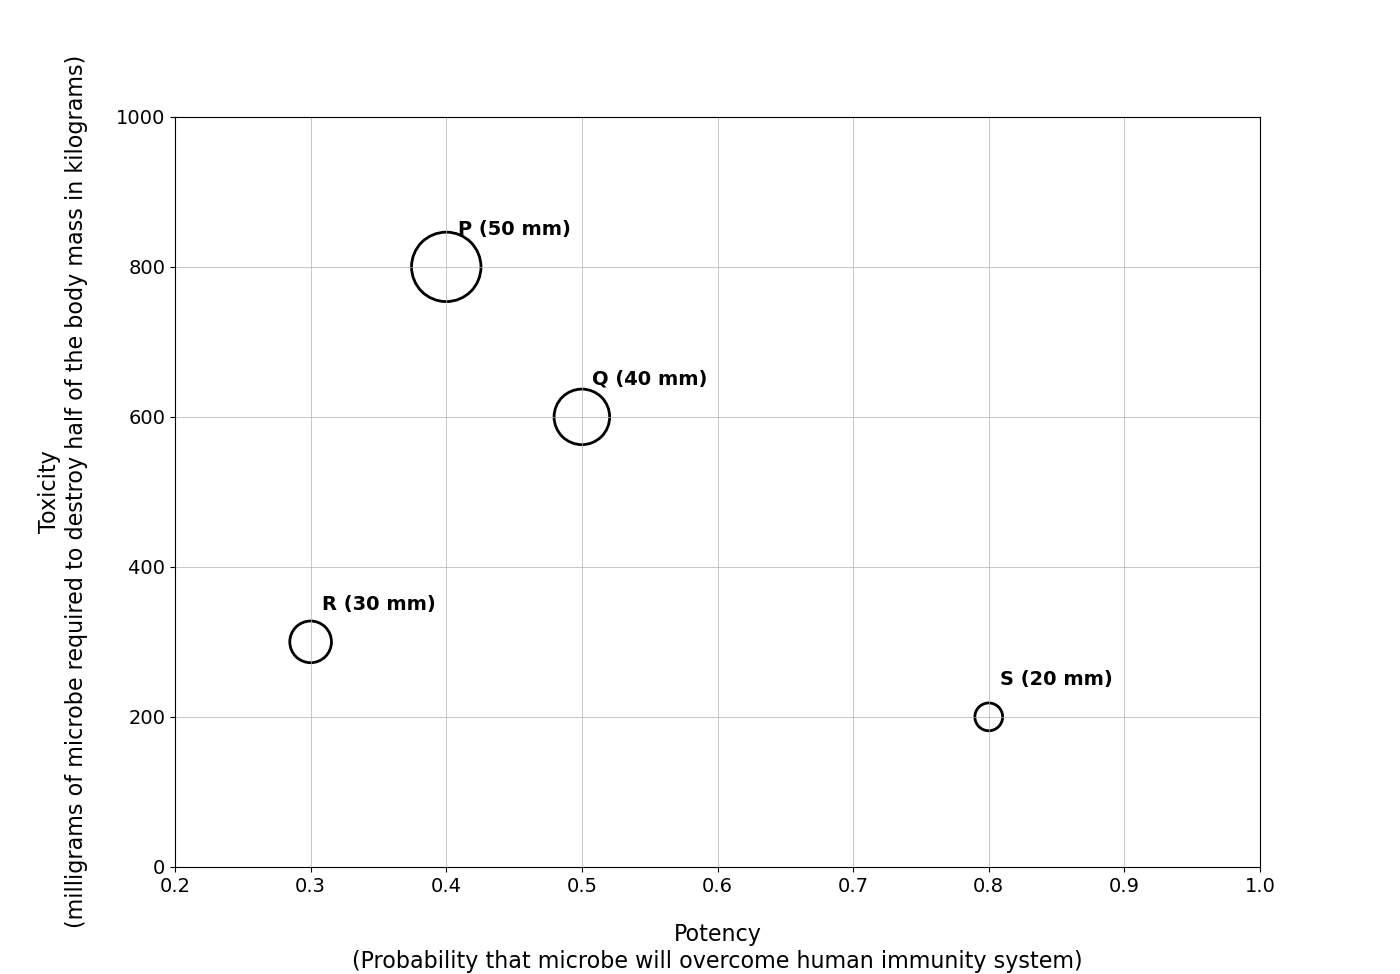
\includegraphics[width=0.5\linewidth]{figs/Figure_1.png}
    \label{fig:enter-label}
\end{figure}
A pharmaceutical company is contemplating the development of a vaccine against the most dangerous microbe. Which microbe should the company target in its first attempt?
\begin{enumerate}
\begin{multicols}{4}
\item $P$
\item $Q$
\item $R$
\item $S$
\end{multicols}
\end{enumerate}
%62
\item \textbf{Few school curricula include a unit on how to deal with bereavement and grief, and yet all students at some point in their lives suffer from losses through death and parting.}\\
Based on the above passage which topic would not be included in a unit on bereavement?\\
\begin{enumerate}
    \item how to write a letter of condolence
    \item what emotional stages are passed through in the healing process
    \item what the leading causes of death are
    \item how to give support to a grieving friend
\end{enumerate}
%63
\item A container originally contains $10$ litres of pure spirit. From this container $1$ litre of spirit is replaced with $1$ litre of water. Subsequently, $1$ litre of the mixture is again replaced with $1$ litre of water and this process is replaced one more time. How much spirit is now left in the container?
\begin{enumerate}
\begin{multicols}{4}
\item $7.58$ litres
\item $7.84$ litres
\item $7$ litres
\item $7.29$ litres
\end{multicols}
\end{enumerate}
%64
\item A transporter receives the same number of orders each day. Currently, he has some pending orders $\brak{\text{backlog}}$ to be shipped. If he uses $7$ trucks, then at the end of the $4$th day he can clear all the orders. Alternatively, if he uses only $3$ trucks, then all the orders are cleared at the end of the $10$th day. What is the minimum number of trucks required so that there will be no pending order at the end of the $5$th day?
\begin{enumerate}
\begin{multicols}{4}
\item 4
\item 5
\item 6
\item 7
\end{multicols}
\end{enumerate}
%65
\item The variable cost $\brak{V}$ of manufacturing a product varies according to the equation $V=4q$, where $q$ is the quantity produced. The fixed cost $\brak{F}$ of production of same product reduces with $q$ according to the equation $F=\frac{100}{q}$. How many units should be produced to minimize the total cost $\brak{V+F}$?
\begin{enumerate}
\begin{multicols}{4}
\item 5
\item 4
\item 7
\item 6
\end{multicols}
\end{enumerate}
\end{enumerate}
\end{document}
